\subsection{Эллипсы рассеивания}
\noindent Для уравнения эллипса выбиралась константа равная $const = 2 \cdot (2 \cdot \sigma)$

	\begin{figure}[H]
		\centering
		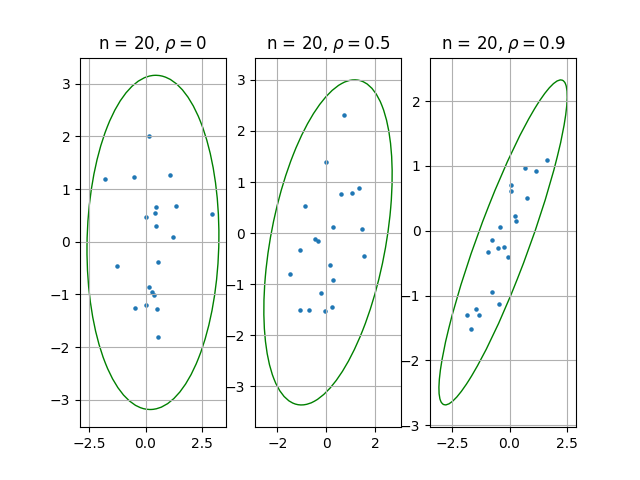
\includegraphics[width = 13cm, height = 8cm]{part_scattering_ellipse/figures/n_20}
		\caption{Двумерное нормальное распределение, $n$ = 20}
		\label{fig:n20}
	\end{figure}

	\begin{figure}[H]
		\centering
		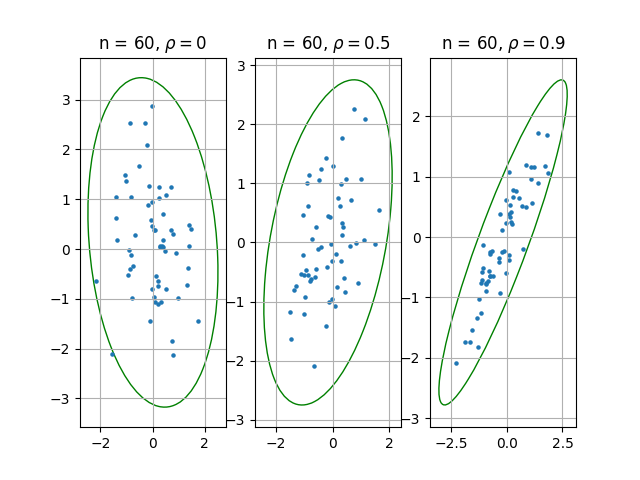
\includegraphics[width = 13cm, height = 8cm]{part_scattering_ellipse/figures/n_60}
		\caption{Двумерное нормальное распределение, $n$ = 60}
		\label{fig:n60}
	\end{figure}

	\begin{figure}[H]
		\centering
		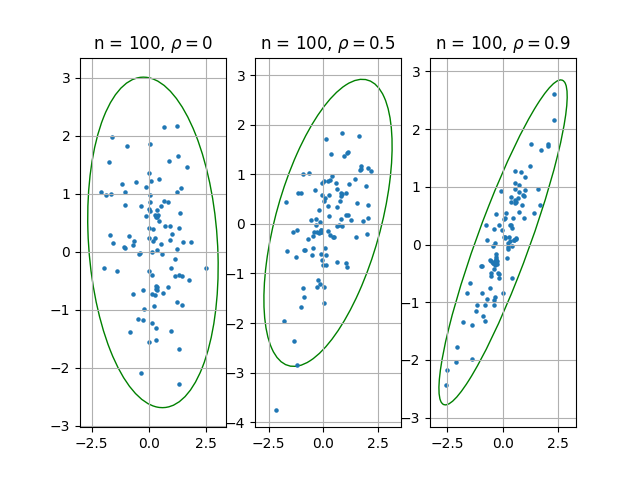
\includegraphics[width = 13cm, height = 8cm]{part_scattering_ellipse/figures/n_100}
		\caption{Двумерное нормальное распределение, $n$ = 100}
		\label{fig:n100}
	\end{figure}